% Options for packages loaded elsewhere
\PassOptionsToPackage{unicode}{hyperref}
\PassOptionsToPackage{hyphens}{url}
%
\documentclass[
]{article}
\usepackage{amsmath,amssymb}
\usepackage{iftex}
\ifPDFTeX
  \usepackage[T1]{fontenc}
  \usepackage[utf8]{inputenc}
  \usepackage{textcomp} % provide euro and other symbols
\else % if luatex or xetex
  \usepackage{unicode-math} % this also loads fontspec
  \defaultfontfeatures{Scale=MatchLowercase}
  \defaultfontfeatures[\rmfamily]{Ligatures=TeX,Scale=1}
\fi
\usepackage{lmodern}
\ifPDFTeX\else
  % xetex/luatex font selection
\fi
% Use upquote if available, for straight quotes in verbatim environments
\IfFileExists{upquote.sty}{\usepackage{upquote}}{}
\IfFileExists{microtype.sty}{% use microtype if available
  \usepackage[]{microtype}
  \UseMicrotypeSet[protrusion]{basicmath} % disable protrusion for tt fonts
}{}
\makeatletter
\@ifundefined{KOMAClassName}{% if non-KOMA class
  \IfFileExists{parskip.sty}{%
    \usepackage{parskip}
  }{% else
    \setlength{\parindent}{0pt}
    \setlength{\parskip}{6pt plus 2pt minus 1pt}}
}{% if KOMA class
  \KOMAoptions{parskip=half}}
\makeatother
\usepackage{xcolor}
\usepackage[margin=1in]{geometry}
\usepackage{color}
\usepackage{fancyvrb}
\newcommand{\VerbBar}{|}
\newcommand{\VERB}{\Verb[commandchars=\\\{\}]}
\DefineVerbatimEnvironment{Highlighting}{Verbatim}{commandchars=\\\{\}}
% Add ',fontsize=\small' for more characters per line
\usepackage{framed}
\definecolor{shadecolor}{RGB}{248,248,248}
\newenvironment{Shaded}{\begin{snugshade}}{\end{snugshade}}
\newcommand{\AlertTok}[1]{\textcolor[rgb]{0.94,0.16,0.16}{#1}}
\newcommand{\AnnotationTok}[1]{\textcolor[rgb]{0.56,0.35,0.01}{\textbf{\textit{#1}}}}
\newcommand{\AttributeTok}[1]{\textcolor[rgb]{0.13,0.29,0.53}{#1}}
\newcommand{\BaseNTok}[1]{\textcolor[rgb]{0.00,0.00,0.81}{#1}}
\newcommand{\BuiltInTok}[1]{#1}
\newcommand{\CharTok}[1]{\textcolor[rgb]{0.31,0.60,0.02}{#1}}
\newcommand{\CommentTok}[1]{\textcolor[rgb]{0.56,0.35,0.01}{\textit{#1}}}
\newcommand{\CommentVarTok}[1]{\textcolor[rgb]{0.56,0.35,0.01}{\textbf{\textit{#1}}}}
\newcommand{\ConstantTok}[1]{\textcolor[rgb]{0.56,0.35,0.01}{#1}}
\newcommand{\ControlFlowTok}[1]{\textcolor[rgb]{0.13,0.29,0.53}{\textbf{#1}}}
\newcommand{\DataTypeTok}[1]{\textcolor[rgb]{0.13,0.29,0.53}{#1}}
\newcommand{\DecValTok}[1]{\textcolor[rgb]{0.00,0.00,0.81}{#1}}
\newcommand{\DocumentationTok}[1]{\textcolor[rgb]{0.56,0.35,0.01}{\textbf{\textit{#1}}}}
\newcommand{\ErrorTok}[1]{\textcolor[rgb]{0.64,0.00,0.00}{\textbf{#1}}}
\newcommand{\ExtensionTok}[1]{#1}
\newcommand{\FloatTok}[1]{\textcolor[rgb]{0.00,0.00,0.81}{#1}}
\newcommand{\FunctionTok}[1]{\textcolor[rgb]{0.13,0.29,0.53}{\textbf{#1}}}
\newcommand{\ImportTok}[1]{#1}
\newcommand{\InformationTok}[1]{\textcolor[rgb]{0.56,0.35,0.01}{\textbf{\textit{#1}}}}
\newcommand{\KeywordTok}[1]{\textcolor[rgb]{0.13,0.29,0.53}{\textbf{#1}}}
\newcommand{\NormalTok}[1]{#1}
\newcommand{\OperatorTok}[1]{\textcolor[rgb]{0.81,0.36,0.00}{\textbf{#1}}}
\newcommand{\OtherTok}[1]{\textcolor[rgb]{0.56,0.35,0.01}{#1}}
\newcommand{\PreprocessorTok}[1]{\textcolor[rgb]{0.56,0.35,0.01}{\textit{#1}}}
\newcommand{\RegionMarkerTok}[1]{#1}
\newcommand{\SpecialCharTok}[1]{\textcolor[rgb]{0.81,0.36,0.00}{\textbf{#1}}}
\newcommand{\SpecialStringTok}[1]{\textcolor[rgb]{0.31,0.60,0.02}{#1}}
\newcommand{\StringTok}[1]{\textcolor[rgb]{0.31,0.60,0.02}{#1}}
\newcommand{\VariableTok}[1]{\textcolor[rgb]{0.00,0.00,0.00}{#1}}
\newcommand{\VerbatimStringTok}[1]{\textcolor[rgb]{0.31,0.60,0.02}{#1}}
\newcommand{\WarningTok}[1]{\textcolor[rgb]{0.56,0.35,0.01}{\textbf{\textit{#1}}}}
\usepackage{graphicx}
\makeatletter
\def\maxwidth{\ifdim\Gin@nat@width>\linewidth\linewidth\else\Gin@nat@width\fi}
\def\maxheight{\ifdim\Gin@nat@height>\textheight\textheight\else\Gin@nat@height\fi}
\makeatother
% Scale images if necessary, so that they will not overflow the page
% margins by default, and it is still possible to overwrite the defaults
% using explicit options in \includegraphics[width, height, ...]{}
\setkeys{Gin}{width=\maxwidth,height=\maxheight,keepaspectratio}
% Set default figure placement to htbp
\makeatletter
\def\fps@figure{htbp}
\makeatother
\setlength{\emergencystretch}{3em} % prevent overfull lines
\providecommand{\tightlist}{%
  \setlength{\itemsep}{0pt}\setlength{\parskip}{0pt}}
\setcounter{secnumdepth}{-\maxdimen} % remove section numbering
\usepackage{amsmath}
\usepackage{mathtools}
\usepackage{amsthm}
\usepackage{bm}
\ifLuaTeX
  \usepackage{selnolig}  % disable illegal ligatures
\fi
\IfFileExists{bookmark.sty}{\usepackage{bookmark}}{\usepackage{hyperref}}
\IfFileExists{xurl.sty}{\usepackage{xurl}}{} % add URL line breaks if available
\urlstyle{same}
\hypersetup{
  pdftitle={Time Series Analysis - 478 - Exam 1},
  pdfauthor={Alex Towell (atowell@siue.edu)},
  hidelinks,
  pdfcreator={LaTeX via pandoc}}

\title{Time Series Analysis - 478 - Exam 1}
\author{Alex Towell
(\href{mailto:atowell@siue.edu}{\nolinkurl{atowell@siue.edu}})}
\date{}

\begin{document}
\maketitle

\newcommand{\var}{\operatorname{Var}}
\newcommand{\expect}{\operatorname{E}}
\newcommand{\corr}{\operatorname{Corr}}
\newcommand{\cov}{\operatorname{Cov}}
\newcommand{\ssr}{\operatorname{SSR}}
\newcommand{\se}{\operatorname{SE}}

\newcommand{\mat}[1]{\bm{#1}}
\newcommand{\eval}[2]{\left. #1 \right\vert_{#2}}

\hypertarget{part-1}{%
\section{Part 1}\label{part-1}}

\hypertarget{problem-1.1}{%
\subsection{Problem 1.1}\label{problem-1.1}}

Suppose that \(\bm{Z} \coloneqq (Z_1,Z_2,Z_3)'\) is a random vector with
a mean vector \(\bm{\mu} = \operatorname{E}(\bm{Z}) = (0,1,-1)'\) and a
variance-covariance matrix \[
   \bm{\Sigma} = \operatorname{Var}(\bm{Z}) =
   \begin{pmatrix}
       1    & -0.5 & 0   \\
       -0.5 & 2    & 1.5 \\
       0    & 1.5  & 3   \\
   \end{pmatrix}.
\]

\hypertarget{part-a}{%
\subsubsection{Part (a)}\label{part-a}}

\fbox{Calculate $\operatorname{E}(Z_1 - 3 Z_2 - 2 Z_3)$.}

First, given a matrix \(\bm{A}\), we denote the \((i,j)\)-th element by
\(A_{i j}\). If \(\bm{A}\) is a vector, we simplify this notation and
denote the \(i\)-th element by \(A_i\).

The expectation of \(Z_1 - 3 Z_2 - 2 Z_3\) is given by \begin{align*}
      \operatorname{E}(Z_1 - 3 Z_2 - 2 Z_3) &= \operatorname{E}(Z_1) - \operatorname{E}(3 Z_2) - \operatorname{E}(2 Z_3)\\
      &= \operatorname{E}(Z_1) - 3 \operatorname{E}(Z_2) - 2 \operatorname{E}(Z_3)\\
      &= \mu_1 - 3 \mu_2 - 2 \mu_3.
\end{align*}

It is given that \(\bm{\mu} = (0,1,-1)\) and thus \begin{align*}
   \operatorname{E}(Z_1 - 3 Z_2 - 2 Z_3) &= 0 - 3(1) - 2(-1)\\
      &= 0 - 3 + 2\\
      &= -1.
\end{align*}

\hypertarget{part-b}{%
\subsubsection{Part (b)}\label{part-b}}

\fbox{Calculate $\operatorname{Var}(2 Z_1 + Z_3)$.}

We use the theorems \[
   \operatorname{Var}(X+Y) = \operatorname{Var}(X) + \operatorname{Var}(Y) + 2 \operatorname{Cov}(X,Y),
\] and \[
   \operatorname{Cov}(a X, b Y) = a b \operatorname{Cov}(X,Y).
\] The variance of \(2 Z_1 + Z_3\) is given by \begin{align*}
   \operatorname{Var}(2 Z_1 + Z_3)
      &= \operatorname{Var}(2 Z_1) + \operatorname{Var}(Z_3) + 2 \operatorname{Cov}(2 Z_1,Z_3)\\
      &= 2^2 \operatorname{Var}(Z_1) + \operatorname{Var}(Z_3) + 2 \left(2 \operatorname{Cov}(Z_1,Z_3)\right)\\
      &= 4 \Sigma_{1 1} + \Sigma_{3 3} + 4 \Sigma_{1 3}\\
      &= 4(1) + (3) + 4(0)\\
      &= 7.
\end{align*}

\fbox{
\begin{minipage}{.9\textwidth}
Note to Dr. Q: We observe that since $\Sigma_{1 3} = 0$, $Z_1$ and $Z_3$ are
linearly uncorrelated.
Thus, any function $\operatorname{g}(x,y)$ applied to $Z_1$ and $Z_3$ has
approximate mean
$$
   \operatorname{E}(\operatorname{g}(Z_1,Z_3)) \approx \operatorname{g}(\mu_1,\mu_2) + 
      \left. \frac{\partial^2 \operatorname{g}}{\partial x^2} \right\vert_{\mu_1} \Sigma_{1 1} +
      \left. \frac{\partial^2 \operatorname{g}}{\partial y^2} \right\vert_{\mu_3} \Sigma_{3 3}
$$
and approximate variance
$$
   \operatorname{Var}(\operatorname{g}(Z_1,Z_3)) \approx
      \left(\left. \frac{\partial \operatorname{g}}{\partial x} \right\vert_{\mu_1}\right)^2 \Sigma_{1 1} +
      \left(\left. \frac{\partial \operatorname{g}}{\partial y} \right\vert_{\mu_3}\right)^2 \Sigma_{3 3},
$$
which are \emph{exact} if $\operatorname{g}$ is a linear function.
\end{minipage}
}

\hypertarget{part-c}{%
\subsubsection{Part (c)}\label{part-c}}

\fbox{Calculate $\operatorname{Cov}(3 Z_1 - Z_2, Z_2 + 2 Z_3)$.}

We use the computational variance theorem
\(\operatorname{Cov}(X,Y) = \operatorname{E}(XY) - \operatorname{E}(X)\operatorname{E}(Y)\),
which also means
\(\operatorname{E}(XY) = \operatorname{Cov}(X,Y) + \operatorname{E}(X)\operatorname{E}(Y)\).

The covariance of \(3 Z_1 - Z_2\) and \(Z_2 + 2 Z_3\) is given by
\begin{align*}
   \operatorname{Cov}(3 Z_1 - Z_2, Z_2 + 2 Z_3)
      &= \operatorname{E}\left[(3 Z_1 - Z_2)(Z_2 + 2 Z_3)\right] - \operatorname{E}(3 Z_1 - Z_2)\operatorname{E}(Z_2 + 2 Z_3)\\
      &= \operatorname{E}(3 Z_1 Z_2 + 6 Z_1 Z_3 - Z_2^2 - 2 Z_2 Z_3) - (3 \operatorname{E}(Z_1) - \operatorname{E}(Z_2))(\operatorname{E}(Z_2) - 2 \operatorname{E}(Z_3))\\
      &= 3 \operatorname{E}(Z_1 Z_2) + 6\operatorname{E}(Z_1 Z_3) - \operatorname{E}(Z_2^2) - 2 \operatorname{E}(Z_2 Z_3) - (3 \mu_1 - \mu_2)(\mu_2 - 2 \mu_3).
\end{align*}

Since \(\operatorname{E}(Z_i Z_j) = \Sigma_{i j} + \mu_i \mu_j\), we may
rewrite the above as \[
\begin{split}
   \operatorname{Cov}(3 Z_1 - Z_2, Z_2 + 2 Z_3)
      = 3 (\Sigma_{1 2} + \mu_1 \mu_2) & + 6(\Sigma_{1 3} + \mu_1 \mu_3) - (\Sigma_{2 2} + \mu_2^2) - 2 (\Sigma_{2 3} + \mu_2 \mu_3)\\
      &- (3 \mu_1 - \mu_2)(\mu_2 - 2 \mu_3).
\end{split}
\] We are given the values of \(\Sigma_{i j}\) and \(\mu_i\) for
\(i,j \in \{1,2,3\}\). We may rewrite the above by making these
substitutions, \[
\begin{split}
   \operatorname{Cov}(3 Z_1 - Z_2, Z_2 + 2 Z_3)
      = 3 (-0.5 + 0 \cdot 1) & + 6(0 + 0\cdot(-1)) - (2 + 1^2) - \\
      &2 (1.5 + 1 (-1)) - (3 \cdot 0 - 1)(1 - 2 (-1)).
\end{split}
\] The final calculation results in \[
   \operatorname{Cov}(3 Z_1 - Z_2, Z_2 + 2 Z_3) = -3/2 - 3 - 1 + 3 = -3/2 - 2/2 = -5/2.
\]

\hypertarget{problem-1.2}{%
\subsection{Problem 1.2}\label{problem-1.2}}

Let \(\{e_t\}\) be a normal white noise process with mean zero and
variance \(\sigma^2\). Consider the process \(Y_t = e_t e_{t-1}\).

\hypertarget{part-a-1}{%
\subsubsection{Part (a)}\label{part-a-1}}

\fbox{Calculate $\operatorname{E}(Y_t)$ and $\operatorname{Var}(Y_t)$.}

The expectation of \(Y_t\) is given by \[
   \operatorname{E}(Y_t) = \operatorname{E}(e_t e_{t-1}).
\] By independence, \(\operatorname{E}(Y_t)\) may be rewritten as \[
   \operatorname{E}(Y_t) = \operatorname{E}(e_t) \operatorname{E}(e_{t-1}) = 0.
\]

The variance of \(Y_t\) is given by \[
   \operatorname{Var}(Y_t) = \operatorname{E}(Y_t^2) - \operatorname{E}^2(Y_t).
\] We showed that \(\operatorname{E}(Y_t) = 0\), thus the variance of
\(Y_t\) may be rewritten as \[
   \operatorname{Var}(Y_t) = \operatorname{E}((e_t e_{t-1})^2) = \operatorname{E}(e_t^2 e_{t-1}^2).
\] Since \(e_t\) and \(e_{t-1}\) are independent, \(e_t^2\) and
\(e_{t-1}^2\) are independent, and thus the variance of \(Y_t\) may be
rewritten as \[
   \operatorname{Var}(Y_t) = \operatorname{E}(e_t^2) \operatorname{E}(e_{t-1}^2) = (\sigma^2 + 0)(\sigma^2 + 0) = \sigma^4.
\] We observe that \(\{Y_t\}\) has constant mean \(0\) and constant
variance \(\sigma^4\).

\hypertarget{part-b-1}{%
\subsubsection{Part (b)}\label{part-b-1}}

\fbox{Calculate the ACF (autocorrelation function).}

The autocovariance of \(Y_t\) and \(Y_{t-\ell}\), \(\ell \geq 0\), is
given by \[
   \operatorname{Cov}(Y_t,Y_{t-\ell}) = \operatorname{E}(Y_t Y_{t-\ell}) - \operatorname{E}(Y_t) \operatorname{E}(Y_{t-\ell}).
\] We have already shown in part (a) that \(\operatorname{E}(Y_k) = 0\)
for any \(k\), thus \[
   \operatorname{Cov}(Y_t,Y_{t-\ell}) = \operatorname{E}(Y_t Y_{t-\ell}).
\] Substituting the definition of \(Y_t\) and \(Y_{t-\ell}\) into the
above covariance gives \[
   \operatorname{Cov}(Y_t,Y_{t-\ell}) = \operatorname{E}(e_t e_{t-1} e_{t-\ell} e_{t - \ell - 1}).
\] We perform a case analysis to derive the autocovariance for different
values of \(\ell\).

If \(\ell=0\), then
\(\operatorname{Cov}(Y_t,Y_t) = \operatorname{Var}(Y_t) = \sigma^4\).

If \(\ell=1\), then
\(\operatorname{Cov}(Y_t,Y_{t-1}) = \operatorname{E}(e_t e_{t-1} e_{t-1} e_{t-2})\).
Let \(W \coloneqq e_{t-1}^2\), in which case
\(\operatorname{Cov}(Y_t,Y_{t-1}) = \operatorname{E}(e_t W e_{t-2})\).
Since these are independent random variables, \[
   \operatorname{Cov}(Y_t,Y_{t-1}) = \operatorname{E}(e_t) \operatorname{E}(W) \operatorname{E}(e_{t-2}) = 0 \cdot \operatorname{E}(W) \cdot 0 = 0.
\]

If \(\ell=2\), then \[
   \operatorname{Cov}(Y_t,Y_{t-2}) = \operatorname{E}(e_t e_{t-1} e_{t-2} e_{t-3}).
\] Since these are independent random variables, \[
   \operatorname{Cov}(Y_t,Y_{t-1}) = \operatorname{E}(e_t) \operatorname{E}(e_{t-1}) \operatorname{E}(e_{t-2}) \operatorname{E}(e_{t-3}) = 0.
\] Any \(\ell \geq 2\) resutls in two elements of \(\{Y_t\}\) that have
no random noise elements in common and thus also have a covariance of
zero.

Since the autocovariance function is symmetric about \(t\),
\(\operatorname{Cov}(Y_t,Y_{t+\ell}) = \operatorname{Cov}(Y_t,Y_{t-\ell})\),
and thus we see that the autocovariance function is strictly a function
of the lag \(\ell\).

We reparameterize the autocovariance function \(\gamma\) with respect to
\(\ell\), \[
   \gamma_\ell =
   \begin{cases}
      \sigma^4    & \ell = 0\\
      0           & \ell \neq 0.
   \end{cases}
\] The autocorrelation function ls\(\rho_\ell\) is defined as
\(\gamma_\ell / \gamma_0\), thus \[
   \rho_\ell =
   \begin{cases}
      1    & \ell = 0\\
      0    & \ell \neq 0.
   \end{cases}
\]

\hypertarget{part-c-1}{%
\subsubsection{Part (c)}\label{part-c-1}}

\fbox{Is the process weakly stationary? Why?}

The process is weakly stationary. It is weakly stationary because its
mean is a constant \(0\), its variance is a constant \(\sigma^4\), and
its autocorrelation function is strictly a function of lag \(\ell\).

\hypertarget{problem-1.3}{%
\subsection{Problem 1.3}\label{problem-1.3}}

\fbox{
\begin{minipage}{.9\textwidth}
Suppose that we have fit the straight-line regression without intercept $\hat y = \hat\beta_1 x_1$.
However, the response $y$ is in fact affected by a second variable $x_2$.
So the true regression function is
$$
   y = \beta_1 x_1 + \beta_2 x_2 + \epsilon.
$$
Assume $\epsilon$’s are i.i.d. with mean $0$ and variance $\sigma^2$.
Calculate the bias of $\hat\beta_1$ in the original simple linear regression,
i.e. calculate $\operatorname{E}(\hat\beta_1-\beta_1)$.
\end{minipage}}

First, we find an estimator \(\hat\beta_1\) given a random sample
\(\{Y_i\}\) generated from the model \[
   Y_i = \beta_1 x_{i 1} + \beta_2 x_{i 2} + \epsilon_i,
\] except we incorrectly or approximately assume
\(Y_i = \beta_1 x_{i 1} + \epsilon_i\). The true statistical error of
the \(i\)-th random variable \(Y_i\) is given by \[
   \epsilon_i = Y_i - \beta_1 x_{i 1} - \beta_2 x_{i 2}
\] and we are interested in minimizing the sum of the squares of the
statistical errors \[
   \operatorname{L} = \sum_{i=1}^{n} \epsilon_i^2.
\] We (incorrectly or approximately) assume
\(\epsilon_i = Y_i - \beta_1 x_{i 1}\) and parameterize
\(\operatorname{L}\) with respect to \(\beta_1\), resulting in the
function \[
   \operatorname{L}(\beta_1) = \sum_{i=1}^n (Y_i - \beta_1 x_{i 1})^2.
\] We obtain an estimator for \(\beta_1\) by solving for
\(\hat{\beta_1}\) in \[
   \left. \frac{\partial \operatorname{L}}{\partial \beta_1} \right\vert_{\hat{\beta_1}}= 0.
\] Thus, \begin{align*}
         -2 \sum_i (Y_i - \hat\beta_1 x_{i 1}) x_{i 1} &= 0\\
         \sum_i \left(Y_i x_{i 1} - \hat\beta_1 x_{i 1}^2 \right) &= 0\\
         \hat\beta_1 \sum_i x_{i 1}^2  &= \sum_i Y_i x_{i 1}
\end{align*} which finally simplifies to \[
   \hat\beta_1 = \frac{\sum_{i=1}^n Y_i x_{i 1}}{\sum_{i=1}^n x_{i 1}^2}
\]

We are interested in the bais of \(\hat\beta_1\), denoted by \[
   \operatorname{b}(\hat\beta_1) \coloneqq \operatorname{E}(\hat\beta_1 - \beta_1).
\] By the linearity of expectation, the bias may be rewritten as \[
   \operatorname{b}(\hat\beta_1) = \operatorname{E}(\hat\beta_1) - \beta_1.
\] The expectation of \(\hat\beta_1\) is given by \begin{align*}
   \operatorname{E}(\hat\beta_1)
      &= \operatorname{E}\left(\frac{\sum_i Y_i x_{i 1}}{\sum_i x_{i 1}^2}\right)\\
      &= \frac{\operatorname{E}\left(\sum_i Y_i x_{i 1}\right)}{\sum_i x_{i 1}^2}\\
      &= \frac{\sum_i \operatorname{E}(Y_i x_{i 1})}{\sum_i x_{i 1}^2}\\
      &= \frac{\sum_i x_{i 1} \operatorname{E}(Y_i) }{\sum_i x_{i 1}^2}.
\end{align*} The true model of \(\{Y_i\}\) is given by
\(Y_i = \beta_1 x_{i 1} + \beta_2 x_{i 2} + \epsilon_i\), so
\begin{align*}
   \operatorname{E}(\hat\beta_1)
      &= \frac{\sum_i x_{i 1} \operatorname{E}(\beta_1 x_{i 1} + \beta_2 x_{i 2} + \epsilon_i)}{\sum_i x_{i 1}^2}\\
      &= \frac{\sum_i x_{i 1} (\beta_1 x_{i 1} + \beta_2 x_{i 2})}{\sum_i x_{i 1}^2}\\
      &= \frac{\sum_i \beta_1 x_{i 1}^2 + \beta_2 x_{i 1} x_{i 2}}{\sum_i x_{i 1}^2}\\
      &= \frac{\sum_i \beta_1 x_{i 1}^2}{\sum_i x_{i 1}^2} + \frac{\sum_i \beta_2 x_{i 1} x_{i 2}}{\sum_i x_{i 1}^2}\\
      &= \beta_1 \frac{\sum_i x_{i 1}^2}{\sum_i x_{i 1}^2} + \beta_2 \frac{\sum_i x_{i 1} x_{i 2}}{\sum_i x_{i 1}^2}\\
      &= \beta_1 + \beta_2 \frac{\sum_i x_{i 1} x_{i 2}}{\sum_i x_{i 1}^2}
\end{align*} The bias is defined as
\(\operatorname{b}(\hat\beta_1) = \operatorname{E}(\hat\beta_1) - \beta_1\),
thus \[
   \operatorname{b}(\hat\beta_1) = \beta_2 \frac{\sum_{i=1}^n x_{i 1} x_{i 2}}{\sum_{i=1}^n x_{i 1}^2}.
\]

The bias of \(\hat\beta_1\) is a function of the observed values
\(\{x_{i 1}\}\) and \(\{x_{i 2}\}\) and the magnitude of \(\beta_2\).

\hypertarget{problem-1.4}{%
\subsection{Problem 1.4}\label{problem-1.4}}

Consider the simple linear regression model
\(y = \beta_0 + \beta_1 x + \epsilon\), where \(\beta_0\) is known.
\(\epsilon\)'s are i.i.d. with mean \(0\) and variance \(\sigma^2\).

\hypertarget{part-a-2}{%
\subsubsection{Part (a)}\label{part-a-2}}

\fbox{Find the least square estimator of $\beta_1$ in this model.}

Since \(\beta_0\) is known, we only need to find an estimator for
\(\beta_1\). The least-squares estimator of \(\beta_1\) is defined as

\[
   \hat\beta_1 = {\mathop{\mathrm{argmin}}\limits}_{\beta_1} \operatorname{L}(\beta_1 | \beta_0)
\] where
\(\operatorname{L}(\beta_1 | \beta_0) = \sum_{i=1}^n \left(Y_i - \beta_0 - \beta_1 x_i\right)^2\).
We obtain the estimator by solving for \(\hat\beta_1\) in \[
   \left. \frac{\partial \operatorname{L}}{\partial \beta_1} \right\vert_{\hat\beta_1} = 0.
\]

Thus, \begin{align*}
         -2 \sum_{i=1}^n (Y_i - \beta_0 - \hat\beta_1 x_i)x_i &= 0\\
         \sum_{i=1}^n \left(x_i Y_i - \beta_0 x_i - \hat\beta_1 x_i^2\right) &= 0\\
         \sum_{i=1}^n x_i Y_i - \beta_0 \sum_{i=1}^n x_i - \hat\beta_1 \sum_{i=1}^n x_i^2 &= 0\\
         \hat\beta_1 \sum_{i=1}^n x_i^2  &= \sum_{i=1}^n x_i Y_i - \beta_0 \sum_{i=1}^n x_i,
\end{align*} which finally simplifies to \[
   \hat\beta_1 = \frac{\sum_{i=1}^n x_i Y_i - \beta_0 \sum_{i=1}^n x_i}{\sum_{i=1}^n x_i^2}.
\]

Of course, when \(\{Y_i\} = \{y_i\}\), \(\hat{\beta_1}\) realizes the
particular vlaue \[
   \hat\beta_1 = \frac{\sum_{i=1}^n x_i y_i - \beta_0 \sum_{i=1}^n x_i}{\sum_{i=1}^n x_i^2}.
\]

The expectation of \(\hat\beta_1\) is given by \begin{align*}
   \operatorname{E}(\hat\beta_1)
      &= \operatorname{E}{\frac{\sum_i x_i Y_i - \beta_0 \sum_i x_i}{\sum_i x_i^2}}\\
      &= \left(\sum_i x_i^2\right)^{-1}\operatorname{E}\left(\sum_i x_i Y_i - \beta_0 \sum_i x_i\right)\\
      &= \left(\sum_i x_i^2\right)^{-1}\left(\sum_i x_i \operatorname{E}(\beta_0 + \beta_1 x_i + \epsilon_i) - \beta_0 \sum_i x_i\right)\\
      &= \left(\sum_i x_i^2\right)^{-1}\left(\beta_0 \sum_i x_i + \beta_1 \sum_i x_i^2 - \beta_0 \sum_i x_i\right)\\
      &= \beta_1 \left(\sum_i x_i^2\right)^{-1}\left(\sum_i x_i^2\right)\\
      &= \beta_1,
\end{align*} which shows that it is unbiased (as expected).

\hypertarget{part-b-2}{%
\subsubsection{Part (b)}\label{part-b-2}}

\fbox{
\begin{minipage}{.9\textwidth}
Construct a $100(1-\alpha)\%$ confidence interval for $\beta_1$.
Compare the interval with the one when $\beta_0$ is also unknown.
Is it narrower?
\end{minipage}
}

To construct the confidence interval, we must find the standard
deviation of \(\hat\beta_1\). The variance is given by \begin{align*}
   \operatorname{Var}(\hat\beta_1) &= \operatorname{Var}\left(\frac{\sum_{i=1}^n x_i Y_i - \beta_0 \sum_{i=1}^n x_i}{\sum_{i=1}^n x_i^2}\right)\\
   &= \left(
         \sum_{i=1}^n x_i^2
      \right)^{-2}
      \operatorname{Var}\left(
         \sum_{i=1}^n x_i Y_i - \beta_0 \sum_{i=1}^n x_i
      \right)
\end{align*}

Since \(\beta_0\) and \(x_i\) for \(i=1,\ldots,n\) are constants, the
above simplies to

\begin{align*}
   \operatorname{Var}(\hat\beta_1)
      &= \left(\sum_{i=1}^n x_i^2\right)^{-2}
         \operatorname{Var}\left(\sum_{i=1}^n x_i Y_i\right)\\
      &= \left(\sum_{i=1}^n x_i^2\right)^{-2}
         \sum_{i=1}^n \operatorname{Var}(x_i Y_i)\\
      &= \left(\sum_{i=1}^n x_i^2\right)^{-2}
         \sum_{i=1}^n x_i^2 \operatorname{Var}(Y_i)\\
      &= \left(\sum_{i=1}^n x_i^2\right)^{-2}
         \sum_{i=1}^n x_i^2 \operatorname{Var}(\beta_0 + \beta_1 x_i + \epsilon_i)\\
      &= \left(\sum_{i=1}^n x_i^2\right)^{-2}
         \sum_{i=1}^n x_i^2 \operatorname{Var}(\epsilon_i)\\
      &= \left(\sum_{i=1}^n x_i^2\right)^{-2}
         \sum_{i=1}^n x_i^2 \sigma^2\\
      &= \sigma^2 \left(\sum_{i=1}^n x_i^2\right)^{-2}
         \sum_{i=1}^n x_i^2
\end{align*} which finally yields the result \[
   \operatorname{Var}(\hat\beta_1) = \frac{\sigma^2}{\sum_{i=1}^n x_i^2}.
\] The standard error is therefore \[
   \operatorname{SE}(\hat\beta_1) = \frac{\sigma}{\sqrt{\sum_{i=1}^n x_i^2}}.
\]

Since \(\hat\beta_1\) is a linear combination of standard normal
deviates, \(\hat\beta_1\) is normally distributed with a mean
\(\beta_1\) and a variance \(\operatorname{Var}(\hat\beta_1)\). Thus, a
\(100(1-\alpha)\%\) confidence interval for \(\beta_1\) is \[
   \beta_1 \in \left[\hat\beta_1 - z_{\alpha/2} \operatorname{SE}(\hat\beta_1),\hat\beta_1 + z_{\alpha/2} \operatorname{SE}(\hat\beta_1)\right]
\] or, substituting the expression for the standard deviation, \[
   \beta_1 \in \left[\hat\beta_1 - \frac{z_{\alpha/2} \sigma}{\sqrt{\sum_i x_i^2}}, \hat\beta_1 + \frac{z_{\alpha/2} \sigma}{\sqrt{\sum_i x_i^2}}\right].
\]

To compare this estimator with the estimator for unknown
\(\bm{\beta }= (\beta_0, \beta_1)\), we choose to use the matrix
equations for this part as a demonstration of a simpler alternative
approach. The unbiased least-squares estimator of \(\bm{\beta}\) is
given by \[
   \hat{\bm{\beta}}_f = (\bm{X}' \bm{X})^{-1} \bm{X}' \bm{Y}.
\] where \[
   \bm{X} =
   \begin{pmatrix}
      1 & x_1\\
      1 & x_2\\
      \vdots & \vdots\\
      1 & x_n\\
   \end{pmatrix}
\] and \[
   \bm{Y} =
   \begin{pmatrix}
      Y_1\\
      \vdots\\
      Y_n\\
   \end{pmatrix}.
\] Performing the matrix calculations, we see that \[
   \left(\bm{X}' \bm{X}\right) =\
   \begin{pmatrix}
      n                 &     \sum_i x_i\\
      \sum_i x_i        &     \sum_i x_i^2
   \end{pmatrix}
\] and \[
   \left(\bm{X}' \bm{X}\right)^{-1} =\
   \frac{1}{n \sum_i x_i^2 - \left(\sum_i x_i\right)^2}
   \begin{pmatrix}
      \sum_i x_i^2      &     -\sum_i x_i\\
      -\sum_i x_i        &     n
   \end{pmatrix}
\] The variance-covariance matrix of \(\hat\beta_f\) is therefore \[
   \bm{\Sigma} = \operatorname{Var}(\hat\beta_f) = \sigma^2 \left(\bm{X}' \bm{X}\right)^{-1}
\] and therefore the variance of \(\hat\beta_{1,f}\) is given by
\begin{align*}
   \operatorname{Var}(\hat\beta_{1,f})
      &= \sigma^2 \Sigma_{2 2}\\
      &= \frac{n \sigma^2}{n \sum_i x_i^2 - \left(\sum_i x_i\right)^2}\\
      &= \frac{\sigma^2}{\sum_i x_i^2 - \frac{1}{n}\left(\sum_i x_i\right)^2}\\
\end{align*}

Recall that
\(\operatorname{Var}(\hat\beta_1) = \frac{\sigma^2}{\sum_i x_i^2}\). The
ratio of \(\operatorname{Var}(\hat\beta_1)\) to
\(\operatorname{Var}(\hat\beta_{1,f})\) is therefore \begin{align*}
   w  &= \frac{\sum_i x_i^2 - \frac{1}{n}\left(\sum_i x_i\right)^2}{\sum_i x_i^2}\\
      &= 1 - \frac{\left(\sum_i x_i\right)^2}{\sum_i x_i^2}\\
      &= 1 - \frac{n \bar{x}^2}{\overline{x^2}},
\end{align*} which implies \(0 < w < 1\), i.e.,
\(\operatorname{Var}(\hat\beta_{1,f})\) is larger than
\(\operatorname{Var}(\hat\beta_1)\). In particular, since
\(w = \frac{\operatorname{Var}(\hat\beta_1)}{\operatorname{Var}(\hat\beta_{1,f})}\),
\[
   \sigma_{\hat\beta_1} = \sqrt{w} \sigma_{\hat\beta_{1,f}}
\] and thus we may conclude that the confidence interval for
\(\hat\beta_1\) is a factor \(\sqrt{w}\) as wide as the confidence
interval for \(\hat\beta_{1,f}\), where \(\sqrt{w} < 1\).

It was immediately obvious that knowing the value of \(\beta_0\) should
reduce the uncertainty of \(\beta_1\) given a sample, but I thought this
proof was fairly interesting.

Finally, to answer the question, since a larger variance yields a larger
confidence interval, the confidence interval for \(\hat\beta_1\) is
narrower than the confidence interval for \(\hat\beta_{1,f}\).

\hypertarget{part-2}{%
\section{Part 2}\label{part-2}}

\hypertarget{problem-2.1}{%
\subsection{Problem 2.1}\label{problem-2.1}}

The \texttt{EmployeeData} data set gives the number of employees (in
thousands) for a metal fabricator and one of their primary vendors for
each month over a 5-year period. You may find the data in .txt file on
blackboard and read the data into R using read.table command.

\hypertarget{part-a-3}{%
\subsubsection{Part (a)}\label{part-a-3}}

\fbox{
\begin{minipage}{.9\textwidth}
Fit a simple linear model to the data, where $y_t$ is the number of employees
during time period $t$ at the metal fabricator and $x_t$ is the number of
employees at the vendor.
Report the ANOVA table and summary for the model coefficients.
\end{minipage}}

\begin{Shaded}
\begin{Highlighting}[]
\NormalTok{emp\_data }\OtherTok{\textless{}{-}} \FunctionTok{read.table}\NormalTok{(}\StringTok{"EmployeeData.txt"}\NormalTok{, }\AttributeTok{header=}\ConstantTok{TRUE}\NormalTok{)}

\CommentTok{\# fit a multiple regression model}
\NormalTok{ols.fit }\OtherTok{\textless{}{-}} \FunctionTok{lm}\NormalTok{(metal}\SpecialCharTok{\textasciitilde{}}\NormalTok{vendor, }\AttributeTok{data=}\NormalTok{emp\_data)}

\CommentTok{\# get details from the regression output}
\FunctionTok{summary}\NormalTok{(ols.fit)}
\end{Highlighting}
\end{Shaded}

\begin{verbatim}
## 
## Call:
## lm(formula = metal ~ vendor, data = emp_data)
## 
## Residuals:
##     Min      1Q  Median      3Q     Max 
## -3.2348 -1.2393 -0.0311  1.0022  3.7077 
## 
## Coefficients:
##             Estimate Std. Error t value Pr(>|t|)    
## (Intercept) 2.847911   3.299962   0.863    0.392    
## vendor      0.122442   0.009423  12.994   <2e-16 ***
## ---
## Signif. codes:  0 '***' 0.001 '**' 0.01 '*' 0.05 '.' 0.1 ' ' 1
## 
## Residual standard error: 1.59 on 58 degrees of freedom
## Multiple R-squared:  0.7443, Adjusted R-squared:  0.7399 
## F-statistic: 168.8 on 1 and 58 DF,  p-value: < 2.2e-16
\end{verbatim}

\begin{Shaded}
\begin{Highlighting}[]
\CommentTok{\# get the anova table}
\FunctionTok{anova}\NormalTok{(ols.fit)}
\end{Highlighting}
\end{Shaded}

\begin{verbatim}
## Analysis of Variance Table
## 
## Response: metal
##           Df Sum Sq Mean Sq F value    Pr(>F)    
## vendor     1 426.72  426.72  168.83 < 2.2e-16 ***
## Residuals 58 146.59    2.53                      
## ---
## Signif. codes:  0 '***' 0.001 '**' 0.01 '*' 0.05 '.' 0.1 ' ' 1
\end{verbatim}

\hypertarget{part-b-3}{%
\subsubsection{Part (b)}\label{part-b-3}}

\fbox{
\begin{minipage}{.9\textwidth}
Plot of the number of employees at the fabricator versus the number of employees
at the vendor with the ordinary least squares regression line overlaid.
\end{minipage}}

\begin{Shaded}
\begin{Highlighting}[]
\CommentTok{\# vendor and metal seem to be positively correlated.}
\FunctionTok{with}\NormalTok{(emp\_data,}\FunctionTok{plot}\NormalTok{(vendor,metal))}
\FunctionTok{abline}\NormalTok{(ols.fit)}
\end{Highlighting}
\end{Shaded}

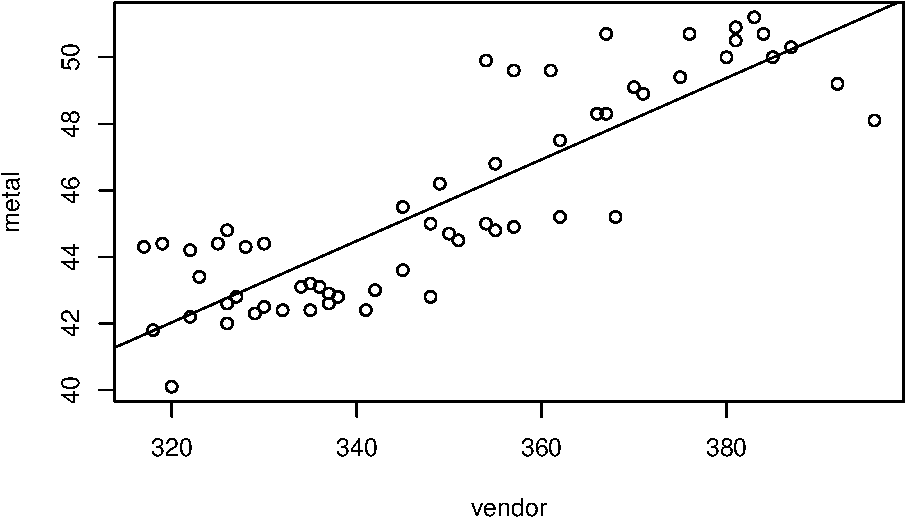
\includegraphics{exam1_files/figure-latex/unnamed-chunk-2-1.pdf}

\begin{Shaded}
\begin{Highlighting}[]
\CommentTok{\#plot(vendor,metal)}
\CommentTok{\#lines(vendor,fitted(ols.fit))}
\end{Highlighting}
\end{Shaded}

\hypertarget{part-c-2}{%
\subsubsection{Part (c)}\label{part-c-2}}

\fbox{
\begin{minipage}{.9\textwidth}
Plot of the residuals versus $t$ (the time ordering).
Does it look random?
\end{minipage}}

Here's the time-ordering plot of the residuals.

\begin{Shaded}
\begin{Highlighting}[]
\NormalTok{N}\OtherTok{=}\FunctionTok{nrow}\NormalTok{(emp\_data)}
\NormalTok{t}\OtherTok{=}\DecValTok{1}\SpecialCharTok{:}\NormalTok{N}
\FunctionTok{plot}\NormalTok{(t,ols.fit}\SpecialCharTok{$}\NormalTok{residual)}
\end{Highlighting}
\end{Shaded}

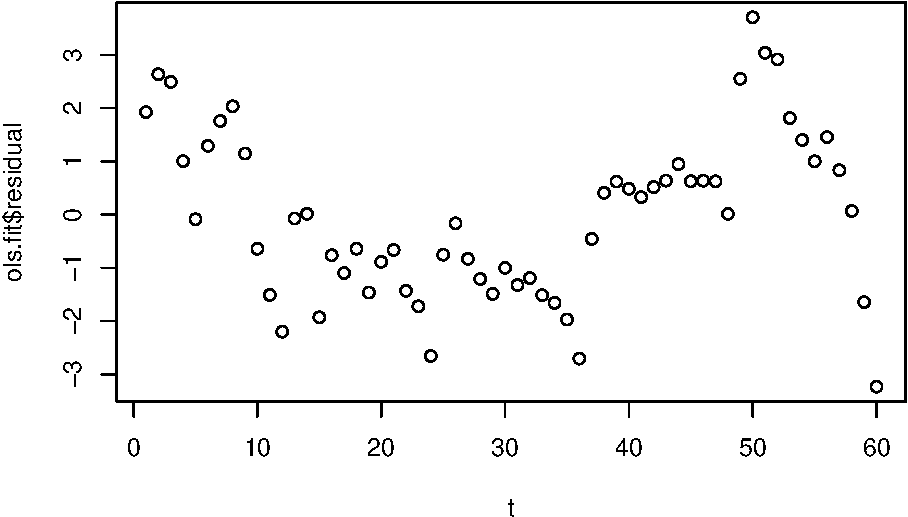
\includegraphics{exam1_files/figure-latex/unnamed-chunk-3-1.pdf}

\begin{Shaded}
\begin{Highlighting}[]
\FunctionTok{acf}\NormalTok{(ols.fit}\SpecialCharTok{$}\NormalTok{residual)}
\end{Highlighting}
\end{Shaded}

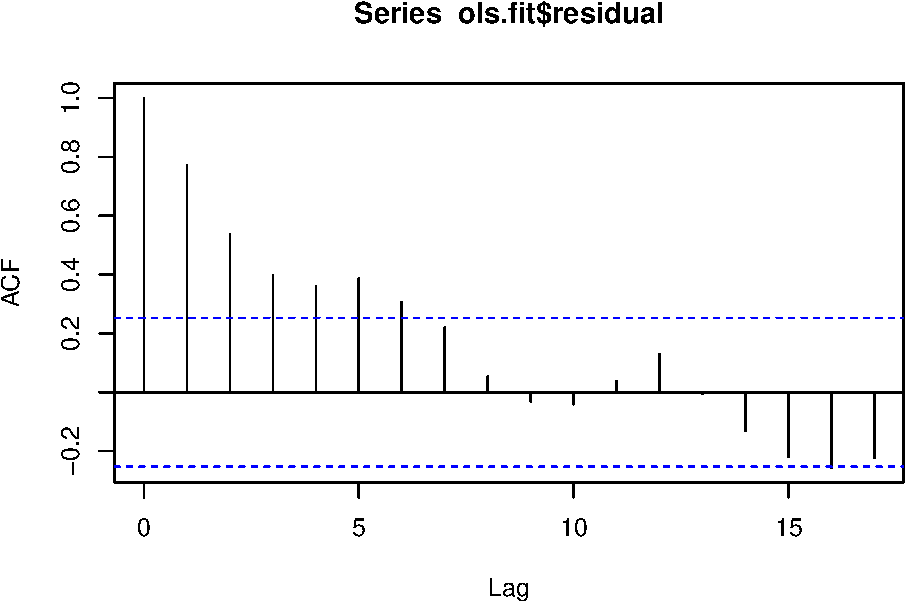
\includegraphics{exam1_files/figure-latex/unnamed-chunk-3-2.pdf}

The residuals do not appear to be i.i.d. normally distributed around
\(0\).

\hypertarget{part-d}{%
\subsubsection{Part (d)}\label{part-d}}

\fbox{
\begin{minipage}{.9\textwidth}
Conduct a Durbin-Watson test to determine the correlation in the residuals.
Comment on your conclusion.
\end{minipage}}

\begin{Shaded}
\begin{Highlighting}[]
\FunctionTok{library}\NormalTok{(}\StringTok{"lmtest"}\NormalTok{)}
\FunctionTok{dwtest}\NormalTok{(ols.fit)}
\end{Highlighting}
\end{Shaded}

\begin{verbatim}
## 
##  Durbin-Watson test
## 
## data:  ols.fit
## DW = 0.35924, p-value < 2.2e-16
## alternative hypothesis: true autocorrelation is greater than 0
\end{verbatim}

\begin{Shaded}
\begin{Highlighting}[]
\CommentTok{\# with(emp\_data,dwtest(metal\textasciitilde{}vendor))}
\end{Highlighting}
\end{Shaded}

If the test statistic \(\rm{DW}\) is around \(2\), there is strong
evidence that there is no autocorrelation. In this case, the statistic
is quite small, and so we have strong evidence to reject the null
hypothesis of no autocorrelation.

\hypertarget{part-e}{%
\subsubsection{Part (e)}\label{part-e}}

\fbox{
\begin{minipage}{.9\textwidth}
Use one iteration of the Cochrane-Orcutt procedure to estimated the regression
coefficients.
Also calculate the standard errors of the coefficients.
Are the standard errors (from the Cochrane-Orcutt procedure) larger than the
ones from simple linear regression?
\end{minipage}}

\begin{Shaded}
\begin{Highlighting}[]
\CommentTok{\# calculte phi fot the Cochrane Method}
\NormalTok{phi.hat}\OtherTok{=}\FunctionTok{lm}\NormalTok{(ols.fit}\SpecialCharTok{$}\NormalTok{residual[}\DecValTok{2}\SpecialCharTok{:}\NormalTok{N]}\SpecialCharTok{\textasciitilde{}}\DecValTok{0}\SpecialCharTok{+}\NormalTok{ols.fit}\SpecialCharTok{$}\NormalTok{residual[}\DecValTok{1}\SpecialCharTok{:}\NormalTok{N}\DecValTok{{-}1}\NormalTok{])}\SpecialCharTok{$}\NormalTok{coeff   }

\CommentTok{\# transform y and x according to the Cochrane Method}
\NormalTok{y.trans}\OtherTok{=}\NormalTok{emp\_data}\SpecialCharTok{$}\NormalTok{metal[}\DecValTok{2}\SpecialCharTok{:}\NormalTok{N]}\SpecialCharTok{{-}}\NormalTok{phi.hat}\SpecialCharTok{*}\NormalTok{emp\_data}\SpecialCharTok{$}\NormalTok{metal[}\DecValTok{1}\SpecialCharTok{:}\NormalTok{N}\DecValTok{{-}1}\NormalTok{]          }
\NormalTok{x.trans}\OtherTok{=}\NormalTok{emp\_data}\SpecialCharTok{$}\NormalTok{vendor[}\DecValTok{2}\SpecialCharTok{:}\NormalTok{N]}\SpecialCharTok{{-}}\NormalTok{phi.hat}\SpecialCharTok{*}\NormalTok{emp\_data}\SpecialCharTok{$}\NormalTok{vendor[}\DecValTok{1}\SpecialCharTok{:}\NormalTok{N}\DecValTok{{-}1}\NormalTok{]}

\CommentTok{\# fit OLS regression with transformed data}
\NormalTok{coch.or}\OtherTok{=}\FunctionTok{lm}\NormalTok{(y.trans}\SpecialCharTok{\textasciitilde{}}\NormalTok{x.trans)     }
\FunctionTok{summary}\NormalTok{(coch.or)}
\end{Highlighting}
\end{Shaded}

\begin{verbatim}
## 
## Call:
## lm(formula = y.trans ~ x.trans)
## 
## Residuals:
##     Min      1Q  Median      3Q     Max 
## -2.1944 -0.4425  0.1461  0.5125  1.2218 
## 
## Coefficients:
##             Estimate Std. Error t value Pr(>|t|)    
## (Intercept)  4.87560    0.78655   6.199 6.78e-08 ***
## x.trans      0.04795    0.01300   3.688 0.000505 ***
## ---
## Signif. codes:  0 '***' 0.001 '**' 0.01 '*' 0.05 '.' 0.1 ' ' 1
## 
## Residual standard error: 0.7342 on 57 degrees of freedom
## Multiple R-squared:  0.1927, Adjusted R-squared:  0.1785 
## F-statistic:  13.6 on 1 and 57 DF,  p-value: 0.0005054
\end{verbatim}

\begin{Shaded}
\begin{Highlighting}[]
\FunctionTok{acf}\NormalTok{(coch.or}\SpecialCharTok{$}\NormalTok{residual)}
\end{Highlighting}
\end{Shaded}

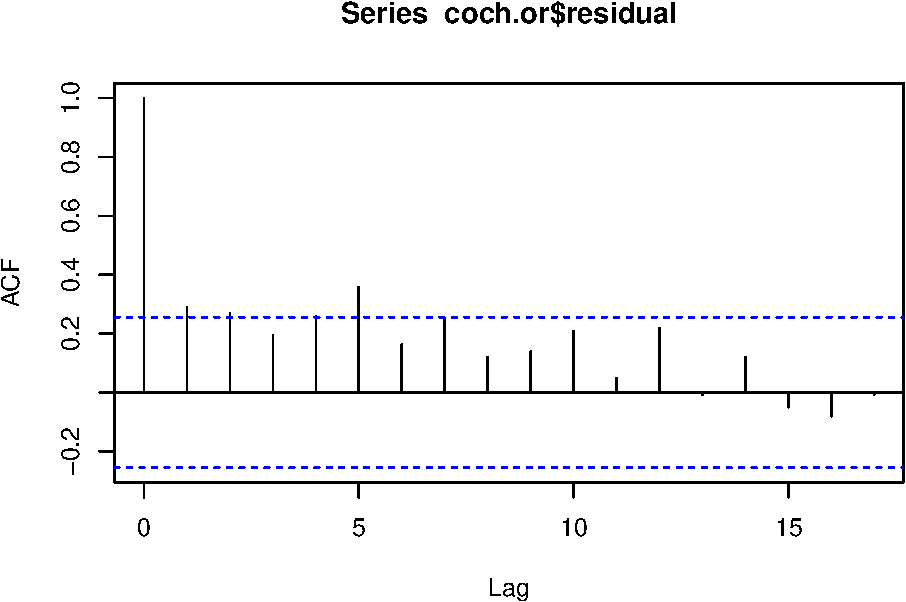
\includegraphics{exam1_files/figure-latex/unnamed-chunk-5-1.pdf}

The standard error of the simple linear regression model for the
intercept was \(3.299962\). The standard error for the intercept in the
Cochrane-Orcutt model is significantly smaller at \(0.78655\).

The standard error of the simpler linear regression model for the slope
is \(0.009423\). The standard error for the intercept in the
Cochrane-Orcutt model is slightly larger at \(0.01300\).

The ACF for the Cochrane-Orcutt fit exhibits far less correlation, most
of the lag times being within the bands.

\hypertarget{problem-2.2}{%
\subsection{Problem 2.2}\label{problem-2.2}}

The following analysis are based on the data in \texttt{HomePrice.txt}
file on blackboard. You may read the data into R using read.table
command. This \texttt{HomePrice} dataset has the following variables:

\begin{enumerate}
\item[-] $Y$ = sale price of home
\item[-] $X_1$ = logged square footage of home
\item[-] $X_2$ = logged square footage of the lot
\end{enumerate}

\hypertarget{part-a-4}{%
\subsubsection{Part (a)}\label{part-a-4}}

\fbox{
\begin{minipage}{.9\textwidth}
Fit an ordinary linear regression model,
$Y = \beta_0 + \beta_1 X_1 + \beta_2 X_2 + \epsilon$.
Report the ANOVA table and summary for the model coefficients.
\end{minipage}}

\begin{Shaded}
\begin{Highlighting}[]
\NormalTok{hp\_data }\OtherTok{\textless{}{-}} \FunctionTok{read.table}\NormalTok{(}\StringTok{"HomePrice.txt"}\NormalTok{, }\AttributeTok{header=}\ConstantTok{TRUE}\NormalTok{)}
\FunctionTok{colnames}\NormalTok{(hp\_data) }\OtherTok{=} \FunctionTok{c}\NormalTok{(}\StringTok{"t"}\NormalTok{,}\StringTok{"Y"}\NormalTok{,}\StringTok{"X1"}\NormalTok{,}\StringTok{"X2"}\NormalTok{)}

\CommentTok{\# fit a multiple regression model}
\NormalTok{hp\_model }\OtherTok{\textless{}{-}} \FunctionTok{lm}\NormalTok{(Y}\SpecialCharTok{\textasciitilde{}}\NormalTok{X1}\SpecialCharTok{+}\NormalTok{X2, }\AttributeTok{data=}\NormalTok{hp\_data)}

\CommentTok{\# get details from the regression output}
\FunctionTok{summary}\NormalTok{(hp\_model)   }
\end{Highlighting}
\end{Shaded}

\begin{verbatim}
## 
## Call:
## lm(formula = Y ~ X1 + X2, data = hp_data)
## 
## Residuals:
##     Min      1Q  Median      3Q     Max 
## -228421  -38178   -5506   25494  383423 
## 
## Coefficients:
##               Estimate Std. Error t value Pr(>|t|)    
## (Intercept) -1.027e+05  1.265e+04  -8.121 3.39e-15 ***
## X1           1.560e+02  4.871e+00  32.019  < 2e-16 ***
## X2           1.151e+00  2.964e-01   3.882 0.000117 ***
## ---
## Signif. codes:  0 '***' 0.001 '**' 0.01 '*' 0.05 '.' 0.1 ' ' 1
## 
## Residual standard error: 78070 on 519 degrees of freedom
## Multiple R-squared:  0.6808, Adjusted R-squared:  0.6796 
## F-statistic: 553.5 on 2 and 519 DF,  p-value: < 2.2e-16
\end{verbatim}

\begin{Shaded}
\begin{Highlighting}[]
\CommentTok{\# get the anova table}
\FunctionTok{anova}\NormalTok{(hp\_model)}
\end{Highlighting}
\end{Shaded}

\begin{verbatim}
## Analysis of Variance Table
## 
## Response: Y
##            Df     Sum Sq    Mean Sq  F value    Pr(>F)    
## X1          1 6.6555e+12 6.6555e+12 1091.875 < 2.2e-16 ***
## X2          1 9.1880e+10 9.1880e+10   15.073 0.0001168 ***
## Residuals 519 3.1635e+12 6.0955e+09                       
## ---
## Signif. codes:  0 '***' 0.001 '**' 0.01 '*' 0.05 '.' 0.1 ' ' 1
\end{verbatim}

\hypertarget{part-b-4}{%
\subsubsection{Part (b)}\label{part-b-4}}

\fbox{Plot of the OLS residuals versus OLS fitted values. Comment on any pattern you see.}

\begin{Shaded}
\begin{Highlighting}[]
\CommentTok{\# studentized residuals}
\NormalTok{r.unweighted }\OtherTok{=} \FunctionTok{rstudent}\NormalTok{(hp\_model)}

\CommentTok{\# the following plot of the fitted values vs the residuals suggests}
\CommentTok{\# non{-}constant variance. the variance seems to be increasing with respect}
\CommentTok{\# to y. the residuals do seem to have a zero mean though.}
\FunctionTok{plot}\NormalTok{(r.unweighted,hp\_model}\SpecialCharTok{$}\NormalTok{fitted)}
\end{Highlighting}
\end{Shaded}

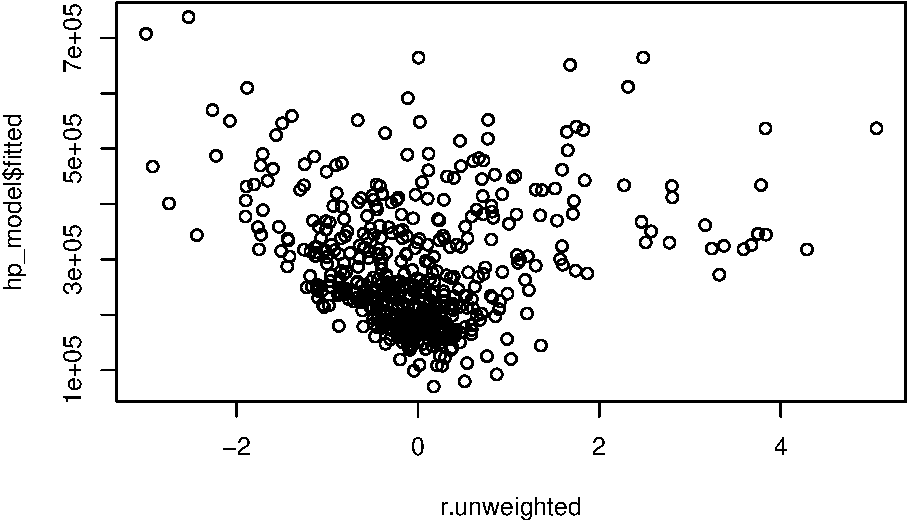
\includegraphics{exam1_files/figure-latex/unnamed-chunk-7-1.pdf}

\begin{Shaded}
\begin{Highlighting}[]
\CommentTok{\# variance seems more constant with respect to home price (X1)}
\FunctionTok{plot}\NormalTok{(r.unweighted,hp\_data}\SpecialCharTok{$}\NormalTok{X1)}
\end{Highlighting}
\end{Shaded}

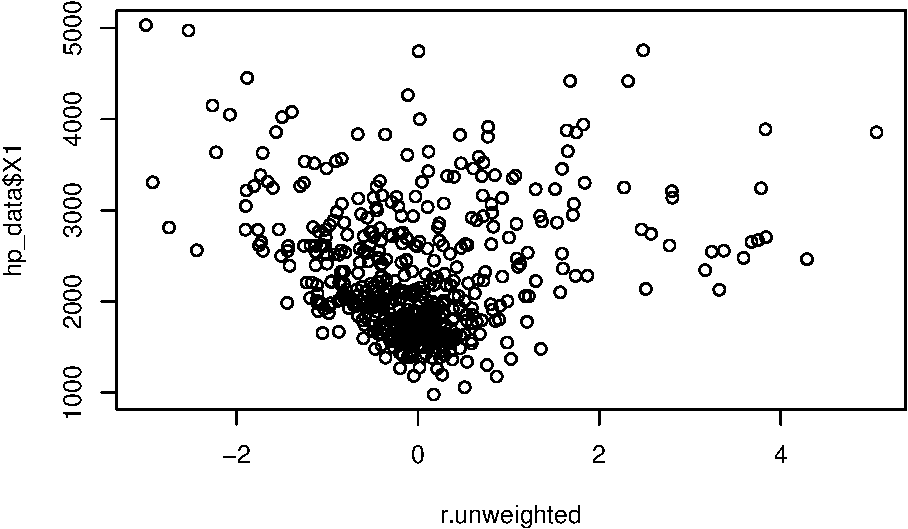
\includegraphics{exam1_files/figure-latex/unnamed-chunk-7-2.pdf}

\begin{Shaded}
\begin{Highlighting}[]
\FunctionTok{plot}\NormalTok{(r.unweighted,hp\_data}\SpecialCharTok{$}\NormalTok{X2)}
\end{Highlighting}
\end{Shaded}

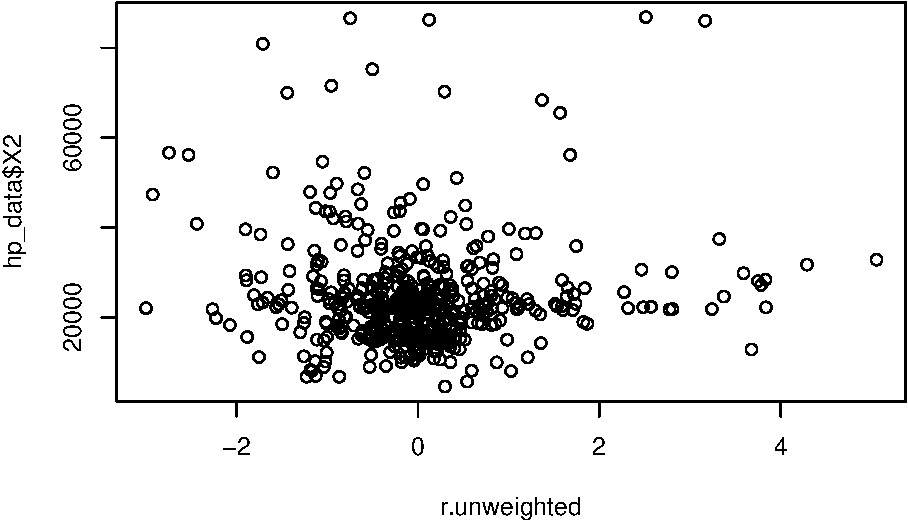
\includegraphics{exam1_files/figure-latex/unnamed-chunk-7-3.pdf}

The studentized residuals of the regression seems to have a non-costant
variance with respect to the fitted values \(\hat{y}\), \(X_1\), and
\(X_2\). Primarily, they exhibit the fanning out characteristic that you
typically see with non-constant variance.

\hypertarget{part-c-3}{%
\subsubsection{Part (c)}\label{part-c-3}}

\fbox{
\begin{minipage}{.9\textwidth}
Calculate the absolute values of the OLS residuals.
Regress the absolute values of the OLS residuals versus the OLS fitted values
and store the fitted values from this regression.
\end{minipage}}

\begin{Shaded}
\begin{Highlighting}[]
\CommentTok{\# the absolute value of the OLS residuals.}
\NormalTok{abs\_residuals }\OtherTok{=} \FunctionTok{abs}\NormalTok{(}\FunctionTok{residuals}\NormalTok{(hp\_model))}

\CommentTok{\# we\textquotesingle{}re fitting}
\CommentTok{\#     s(i) = gamma0 + gamma1 y(i) + zeta(i)}
\CommentTok{\# where zeta(i) is the random error.}
\NormalTok{abs\_residuals\_fit}\OtherTok{=}\FunctionTok{lm}\NormalTok{(abs\_residuals}\SpecialCharTok{\textasciitilde{}}\NormalTok{hp\_model}\SpecialCharTok{$}\NormalTok{fitted)}
\end{Highlighting}
\end{Shaded}

\hypertarget{part-d-1}{%
\subsubsection{Part (d)}\label{part-d-1}}

\fbox{
\begin{minipage}{.9\textwidth}
Calculate weights equal to $1/\hat{e}^2$, where $\hat{e}$ are the fitted values
from the regression in the last step.
Using these weights this time in a weighted least squares regression.
Report the ANOVA table and summary for the model coefficients.
\end{minipage}}

\begin{Shaded}
\begin{Highlighting}[]
\CommentTok{\# weighted least squares. we\textquotesingle{}re taking the squared reciprocal of the estimated}
\CommentTok{\# residuals from the regression model as the weight matrix.}
\NormalTok{wts}\OtherTok{=}\DecValTok{1}\SpecialCharTok{/}\NormalTok{(}\FunctionTok{fitted}\NormalTok{(abs\_residuals\_fit))}\SpecialCharTok{\^{}}\DecValTok{2}

\CommentTok{\# fit the weighted regression model to the data}
\NormalTok{hp\_model.weighted}\OtherTok{=}\FunctionTok{lm}\NormalTok{(Y}\SpecialCharTok{\textasciitilde{}}\NormalTok{X1}\SpecialCharTok{+}\NormalTok{X2, }\AttributeTok{data=}\NormalTok{hp\_data,}\AttributeTok{weights=}\NormalTok{wts)}

\FunctionTok{anova}\NormalTok{(hp\_model.weighted)}
\end{Highlighting}
\end{Shaded}

\begin{verbatim}
## Analysis of Variance Table
## 
## Response: Y
##            Df Sum Sq Mean Sq   F value Pr(>F)    
## X1          1 4095.8  4095.8 1754.0376 <2e-16 ***
## X2          1    0.7     0.7    0.3068 0.5799    
## Residuals 519 1211.9     2.3                     
## ---
## Signif. codes:  0 '***' 0.001 '**' 0.01 '*' 0.05 '.' 0.1 ' ' 1
\end{verbatim}

\begin{Shaded}
\begin{Highlighting}[]
\FunctionTok{summary}\NormalTok{(hp\_model.weighted)}
\end{Highlighting}
\end{Shaded}

\begin{verbatim}
## 
## Call:
## lm(formula = Y ~ X1 + X2, data = hp_data, weights = wts)
## 
## Weighted Residuals:
##     Min      1Q  Median      3Q     Max 
## -9.4644 -0.9364 -0.2118  0.6141  8.0706 
## 
## Coefficients:
##               Estimate Std. Error t value Pr(>|t|)    
## (Intercept) -8918.7876  3619.3749  -2.464   0.0141 *  
## X1            123.1438     3.3186  37.107   <2e-16 ***
## X2             -0.1274     0.2300  -0.554   0.5799    
## ---
## Signif. codes:  0 '***' 0.001 '**' 0.01 '*' 0.05 '.' 0.1 ' ' 1
## 
## Residual standard error: 1.528 on 519 degrees of freedom
## Multiple R-squared:  0.7717, Adjusted R-squared:  0.7708 
## F-statistic: 877.2 on 2 and 519 DF,  p-value: < 2.2e-16
\end{verbatim}

\hypertarget{part-e-1}{%
\subsubsection{Part (e)}\label{part-e-1}}

\fbox{Plot of the WLS residuals versus WLS fitted values. Does it look random now?}

\begin{Shaded}
\begin{Highlighting}[]
\CommentTok{\# weighted residual analysis}

\CommentTok{\# studentized residuals}
\NormalTok{r.weighted }\OtherTok{=} \FunctionTok{rstudent}\NormalTok{(hp\_model.weighted)}

\CommentTok{\# plot studentized residual vs fitted values}
\FunctionTok{plot}\NormalTok{(r.weighted,hp\_model.weighted}\SpecialCharTok{$}\NormalTok{fitted)}
\end{Highlighting}
\end{Shaded}

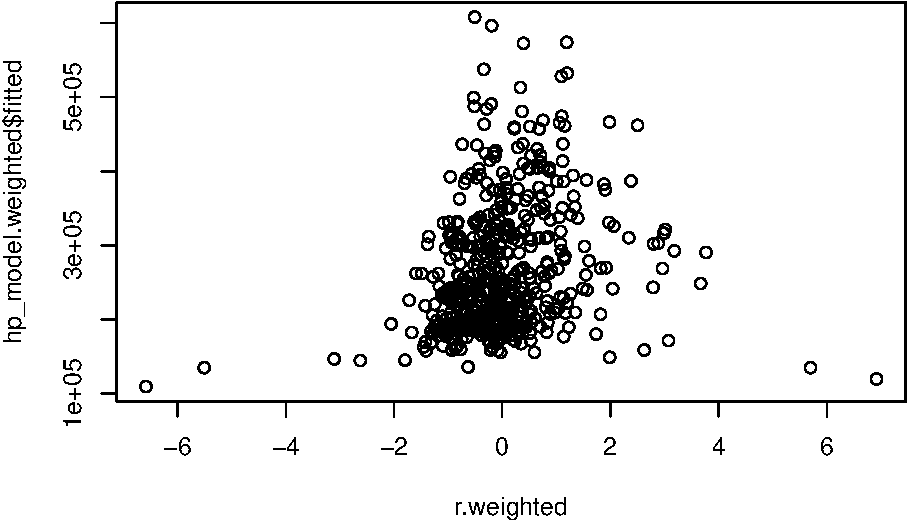
\includegraphics{exam1_files/figure-latex/unnamed-chunk-10-1.pdf}

\begin{Shaded}
\begin{Highlighting}[]
\FunctionTok{plot}\NormalTok{(r.weighted,hp\_data}\SpecialCharTok{$}\NormalTok{X1)}
\end{Highlighting}
\end{Shaded}

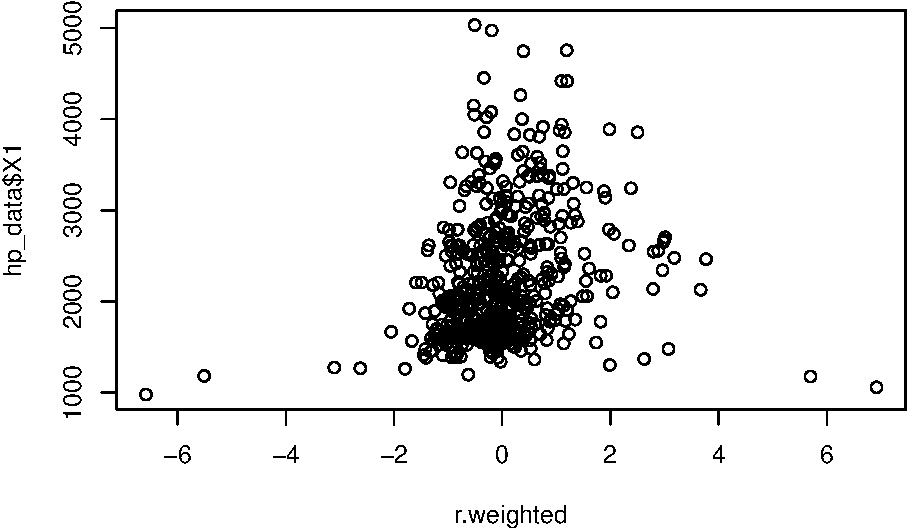
\includegraphics{exam1_files/figure-latex/unnamed-chunk-10-2.pdf}

\begin{Shaded}
\begin{Highlighting}[]
\FunctionTok{plot}\NormalTok{(r.weighted,hp\_data}\SpecialCharTok{$}\NormalTok{X2) }
\end{Highlighting}
\end{Shaded}

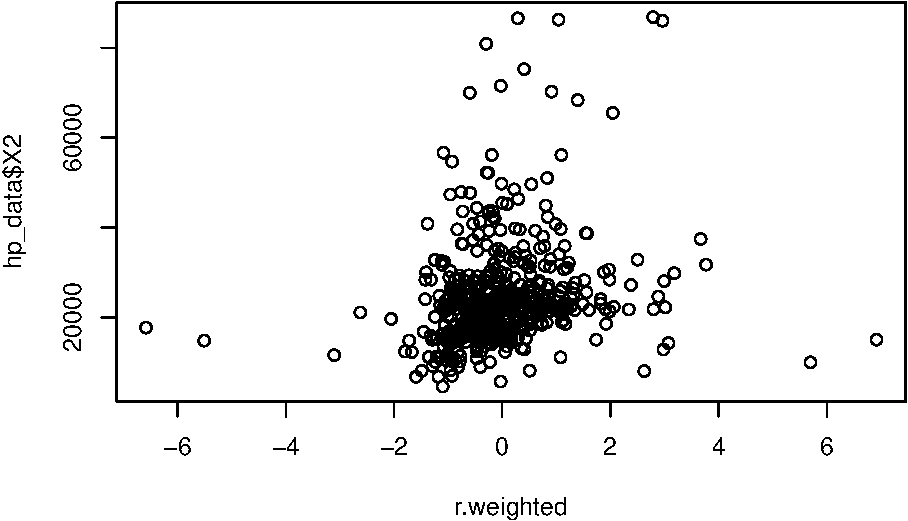
\includegraphics{exam1_files/figure-latex/unnamed-chunk-10-3.pdf}

The studentized residuals of the weighted regression seems to have a
more constant variance with respect to the fitted values \(\hat{y}\),
\(X_1\), and \(X_2\). Primarily, they do not exhibit the fanning out
characteristic that you typically see with non-constant variance.

In conclusion, the weighted regression seems to generate residuals that
are more presentative of random white noise with zero mean and constant
variance.

\end{document}
